\documentclass[12pt,twoside]{article}
\usepackage{amsmath, amssymb}
\usepackage{amsmath}
\usepackage[active]{srcltx}
\usepackage{amssymb}
\usepackage{amscd}
\usepackage{makeidx}
\usepackage{amsthm}
\usepackage{algpseudocode}
\usepackage{algorithm}
\usepackage{listings}
\usepackage{fancyhdr}
\usepackage{graphics}
%----------------------------------------------------------------------------------------------
\usepackage{amsmath, amssymb}
\usepackage{amsmath}
\usepackage[active]{srcltx}
\usepackage{amssymb}
\usepackage{amscd}
\usepackage{makeidx}
\usepackage[dvips]{graphicx}

\renewcommand{\baselinestretch}{1}
\setcounter{page}{1}
\setlength{\textheight}{21.6cm}
\setlength{\textwidth}{14cm}
\setlength{\oddsidemargin}{1cm}
\setlength{\evensidemargin}{1cm}
\pagestyle{myheadings}
\thispagestyle{empty}
\newtheorem{defi}{Definición}
\newtheorem{algoritmo}{Algoritmo}
\markboth{\small{Practica 1. Martínez López Sebastian, Ramírez Resendiz Luis Roque.}}{\small{.}}
\date{}
\begin{document}

\begin{figure}[h]
\vspace{-3cm} \hspace{-2cm} \setlength{\unitlength}{1mm}
\begin{picture}(15,25)(-10,0)

\includegraphics[width=16cm, height=4cm]{TITULO.JPG}
\end{picture}
\end{figure}


\vspace{0cm}

\centerline{\bf Análisis de Algoritmos, Sem: 2023-1, 3CV11, Práctica 1, Fecha: 02 Septiembre 2023}

\centerline{}

%\centerline{}


\begin{center}
\Large{\textsc{Práctica 1: Determinación experimental de la complejidad temporal de un algoritmo}}
\end{center}
\centerline{}
\centerline{\bf {Martinez Lopez Sebastian, Ramirez Resendiz Luis Roque}} 
\centerline{}
\centerline{$sebastian.martinez.lopez98@gmail.com$, $luis\_roque\_ramirez@hotmail.com$}


\bigskip

\textbf{Resumen:} Se realizara el análisis a posteriori y el calculo de la complejidad temporal de los algoritmos propuestos, los cuales son:
\begin{itemize}
\item Algoritmo de búsqueda secuencial entre dos subarreglos de A.
\item Algoritmo de Euclides.
\end{itemize} 

{\bf Palabras Clave:} \textbf{Python, Euclides, Busqueda Secuencial, Arreglos, Subarreglos}.

\section{Introducci\'on}
El uso de los algoritmos tiene una importancia fundamental al momento de desarrollar diversos aplicativos, permitiéndonos optimizar tareas hasta alcanzar que se realicen en el menor tiempo posible, consumiendo a su vez, la menor cantidad de recursos posibles.
Sabemos que cualquier algoritmos es nada mas y nada menos que la transformación de una tarea a una serie de instrucciones finitas y  precisas para que el computador pueda ejecutarlas y que se encuentran presentes en nuestra vida cotidiana, como lo es cuando realizamos alguna receta de cocina, alguna actividad de limpieza como tender nuestra cama entre otros.
Es decir un algoritmo es como un instructivo.
 Por eso, el objetivo principal de esta practica es poder analizar los algoritmos propuestos bajo el estudio de sus complejidades, que pueden ser la espacial S(n), refiriéndose a la cantidad de recursos de memoria, y la complejidad espacial f(n) en la cual nos enfocamos nosotros.
 A su vez, nos enfocamos en ver los datos estadísticos y las diferentes gráficas obtenidas de los mismos en los campos del tiempo de ejecución de los algoritmos propuestos, para a su vez determinar el análisis a posteriori y con esto poder llegar a una conclusión lo mas clara y precisa posible. 

\newpage

\section{Conceptos B\'asicos}
\begin{defi}[Algoritmo]
Acorde a la RAE, podemos definir la palabra algoritmo como "Conjunto ordenado y finito de operaciones que permite hallar la solución de un problema."
Sin embargo podemos complementar dicha informaci\'on tomando en cuenta las partes claves de un algoritmo.
Concluyendo así en otras palabras que un algoritmo es un conjunto de pasos para resolver algo.
\begin{itemize}
\item Preciso: Un algoritmo debe ser claro y conciso para la tarea a realizar.
\item Finito: Un algoritmo no puede ser ejecutado infinitamente.
\item Definido: EL algoritmo debe tener un punto de finalización.
\end{itemize} 

\begin{figure}[h!]
\centering
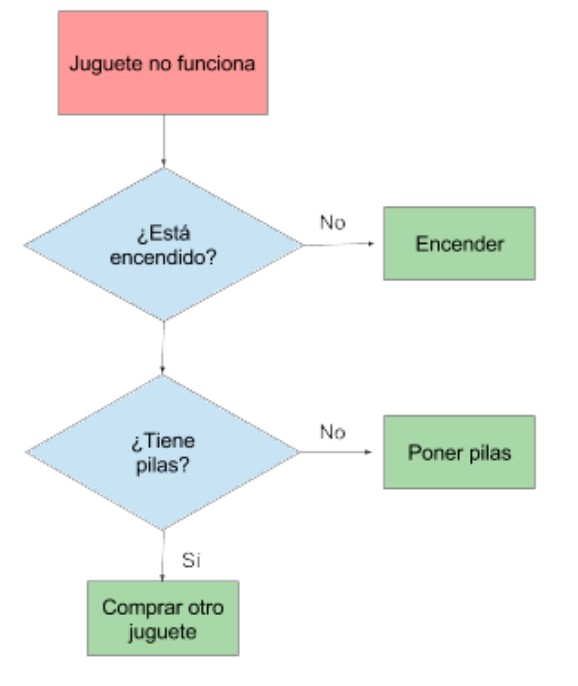
\includegraphics[scale=0.5]{algoritmo.jpg}
\caption{Diagrama de flujo de un algoritmo.}
\label{fig:universe}
\end{figure}
\end{defi}

\clearpage
\begin{defi}[Análisis a posteriori]
Acorde a la RAE, podemos definir la oraci\'on "a posteriori" como  ‘por lo que viene después’. En el ámbito de la filosofía, se emplea para referirse al conocimiento inductivo, esto es, al que se adquiere a partir de la experiencia, ascendiendo de los efectos a las causas.
Así mismo, podemos connotar que el an\'alisis a posteriori se recoge estadísticas de tiempo y espacio consumidas por el algoritmo mientras se ejecuta. 
\end{defi}
\\
\begin{defi}[Notaci\'on O]
Es una herramienta que nos permite determinar la complejidad de un algoritmo determinando su rendimiento en cuanto a recursos y tiempo de ejecución, en pocas palabras nos permite identificar el peor caso donde el algoritmo llegue a su punto mas alto de exigencia.
\\
Así mismo podemos acotar de manera asintótica el crecimiento de un tiempo de ejecución a que este, dentro de factores constante por arriba y por abajo.
\\
Algunos de los términos mas utilizados dentro de la notación Big O son los siguientes:
\\
\begin{figure}[h!]
\centering
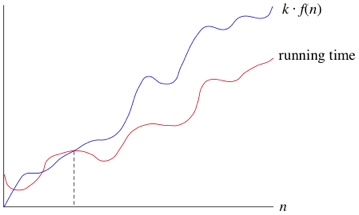
\includegraphics[scale=1.5]{big o.png}
\caption{Definici\'on Big O}
\label{fig:universe}
\end{figure}
\end{defi}
\clearpage
\begin{defi}[Notaci\'on $\Omega$]
Usamos la notación $\Omega$ para representar el limite asintótico inferior del tiempo de una funci\'on, esto quiere decir que, al contrario de la Notaci\'on O, la utilizaremos para calcularla complejidad de un algoritmo en su mejor caso.
\begin{figure}[h!]
\centering
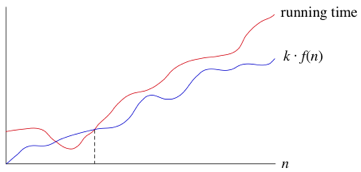
\includegraphics[scale=1.5]{big omega.png}
\caption{Definici\'on $\Omega$}
\label{fig:universe}
\end{figure}
\end{defi}
\begin{defi}[Notaci\'on $\Theta$]
Esta notaci\'on encierra a la funci\'on con un limite superior y un limite inferior. Se puede decir que tenemos una cota asintoticamente ajustada, esto por lo mencionado anteriormente ya que ajustamos el tiempo de ejecuci\'on (funci\'on) dentro del rango de una constante hacia arriba y hacia abajo. Esta notaci\'on se usa para calcular la complejidad de un algoritmo que no tiene mejor ni peor caso

\begin{figure}[h!]
\centering
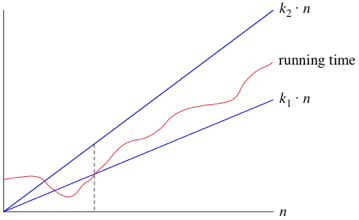
\includegraphics[scale=2.0]{big theta.png}
\caption{Definición $\Theta$}
\label{fig:universe}
\end{figure}
\end{defi}
\clearpage
\begin{algoritmo}[Conjuntos]
Este algoritmo busca crear un conjunto de datos, el cual se almacenara en un arreglo de tamaño N, este arreglo se llenara con datos aleatorios, los cuales van de (0 hasta 3N), lo que se busca es crear dos subconjuntos del arreglo, en otras palabras, se busca crear dos subarreglos partiendo del primero, dividendo el arreglo original en dos, el primero de estos arreglos comenzara del inicio del primer arreglo hasta la mitad, que en este caso es N/2 y el segundo arreglo va de (N/2) +1 es decir una posición mas partiendo de la mitad hacia el final, posteriormente la operación que se realizara es comparar posición a posición del primer subarreglo al cual denominaremos como Arreglo A con el segundo subarreglo, el cual denominaremos como Arreglo B esta comparación se realizara hasta encontrar un valor que se repita en cada uno de los arreglos A y B cuando esto suceda el algoritmo se detendrá y lo próximo que realizara es imprimir el dato que se repite al igual que sus respectivas posiciones, pero estas posiciones serán las que tenga el valor que se repite en el arreglo original, es decir en el arreglo de tamaño N-1, cuando esto pase se terminara la ejecución.
\end{algoritmo}
\begin{figure}[h!]
\centering
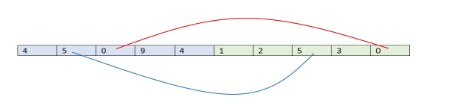
\includegraphics[scale=1.6]{pra1.jpg}
\caption{Arreglo A}
\label{fig:universe}
\end{figure}

\clearpage

\begin{algoritmo}[Euclides]
Euclides, considerado como el padre de la geometría, desarrollo un procedimiento simple  pero  realmente  efectivo  para  calcular  el  máximo  común  divisor  de  dos  números.  Este procedimiento consiste en tomar dos números y dividir el numero mayor entre el menor, siesta división tiene un resultado exacto, entonces el divisor es el m.c.d. En caso contrario,se dividir al divisor entre el resto obtenido, este paso se repite hasta obtener una división exacta. El m.c.d. es el  ́ultimo divisor.
\end{algoritmo}

\begin{figure}[h!]
\centering
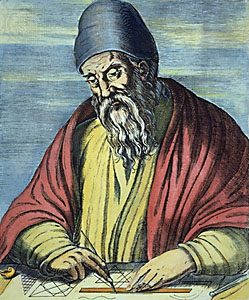
\includegraphics[scale=1.6]{retrato-Euclides-249x300.jpg}
\caption{Euclides}
\label{fig:universe}
\end{figure}

\clearpage

 \section{Experimentaci\'on y Resultados}

\subsection{Ejercicio 1}
Realizar el análisis a posteriori para el mejor y peor caso del algoritmo de conjuntos, en donde el mejor caso es cuando los datos que se repiten se encuentran en las primeras posiciones de cada uno de los sub arreglos, es decir en el Arreglo A y en el Arreglo B. Y el peor caso es cuando no existe ningún dato que se repita. 
\subsubsection{Caso general}
\lstinputlisting[language=Python]{practica.py}
\clearpage

\subsubsection{Grafica del caso general}
\begin{figure}[h!]
\centering
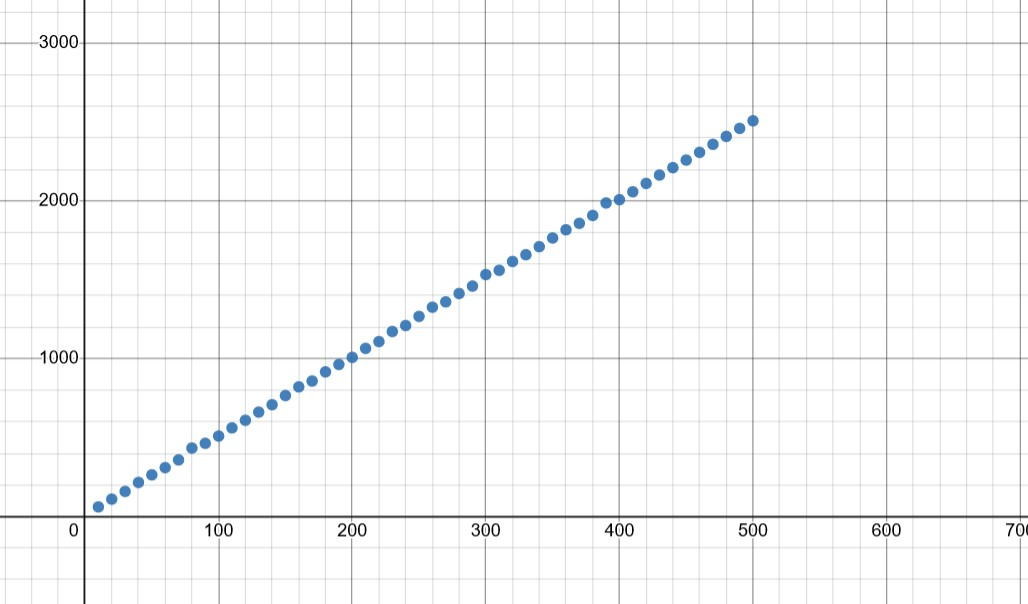
\includegraphics[scale=0.7]{caso_general.jpg}
\caption{Gráfica del caso general}
\label{fig:universe}
\end{figure}
\subsubsection{Tabla de valores}
Asi mismo, estas fueron las coordenadas para graficar el caso general, las cuales estan connotadas por N, que seria el tamaño del arreglo, y ct que seria el contador de las veces que entra en ejecucion el codigo.
\\
\begin{center}
\begin{tabular}{|N|C|}
\hline
N & CT\\
\hline
10 & 61 \\
\hline
20 & 110\\
\hline
30 & 159\\
\hline
40 & 216\\
\hline
50 & 264\\
\hline
60 & 310\\
\hline
70 & 359\\
\hline
80 & 434\\
\hline
90 & 464\\
\hline
100 & 510\\
\hline
  
\end{tabular}
\end{center}
\subsubsection{Mejor Caso}
En este caso, lo unico que hacemos es que forzamos que en la posicion 1 del A1, y en la posicion 1 de A2, se encuentren los mismos valores, para que asi, el algoritmo los encuentre mas rapido, dicho esto, nuesta tabla grafica es la siguiente:
\begin{figure}[h!]
\centering
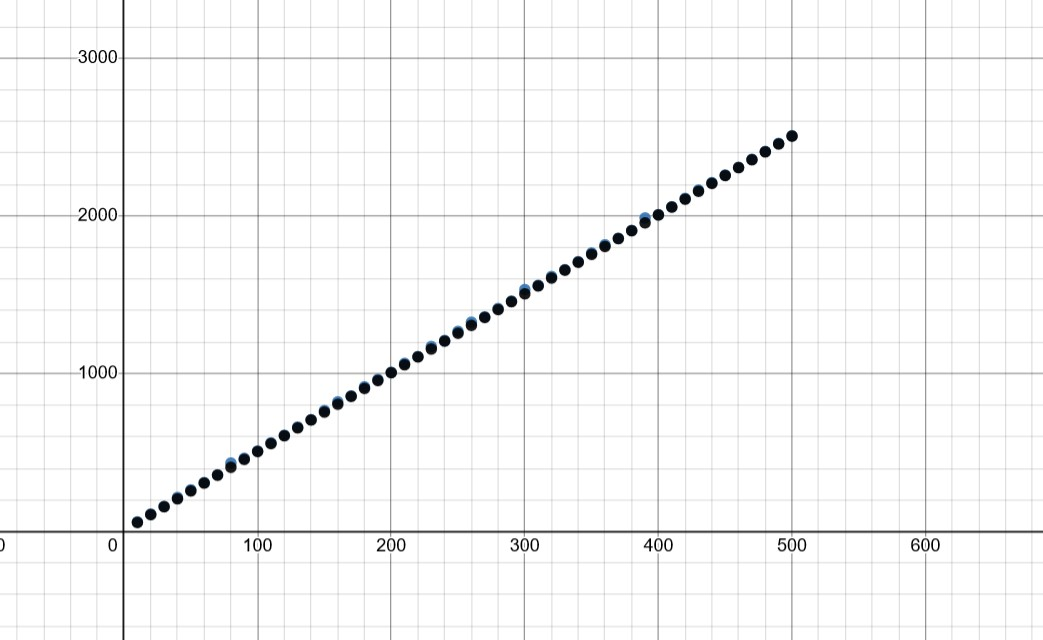
\includegraphics[scale=0.5]{mejor_caso.jpg}
\caption{Gráfica del mejor caso}
\label{fig:universe}
\end{figure}

\subsubsection{Tabla de valores mejor caso}
Asi mismo, estas fueron las coordenadas para graficar el mejor caso, las cuales estan connotadas por N, que seria el tamaño del arreglo, y ct que seria el contador de las veces que entra en ejecucion el codigo.
\begin{center}
\begin{tabular}{|N|C|}
\hline
N & CT\\
\hline
10 & 57\\
\hline
20 & 107\\
\hline
30 & 157\\
\hline
40 & 207\\
\hline
50 & 257\\
\hline
60 & 307\\
\hline
70 & 357\\
\hline
80 & 407\\
\hline
90 & 457\\
\hline
100 & 507\\
\hline

  
\end{tabular}
\end{center}


\subsubsection{Peor Caso}
En este caso, lo único que hacemos es que forzamos que el algoritmo no encuentre ninguna coincidencia, obligandolo asi a que recorra todo el arreglo.
\begin{figure}[h!]
\centering
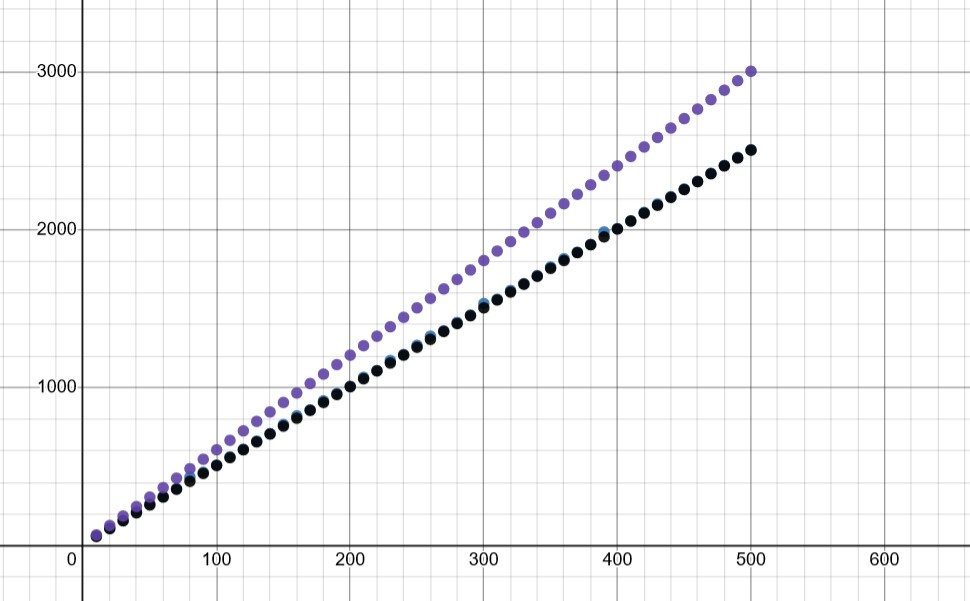
\includegraphics[scale=0.5]{peor_caso.jpg}
\caption{Gráfica del peor caso}
\label{fig:universe}
\end{figure}

\subsubsection{Tabla de valores peor caso}
Asi mismo, estas fueron las coordenadas para graficar el mejor caso, las cuales estan connotadas por N, que seria el tamaño del arreglo, y ct que seria el contador de las veces que entra en ejecucion el codigo.
\begin{center}
\begin{tabular}{|N|C|}
\hline
N & CT\\
\hline
10 & 67\\
\hline
20 & 127\\
\hline
30 & 187\\
\hline
40 & 247\\
\hline
50 & 307\\
\hline
60 & 367\\
\hline
70 & 427\\
\hline
80 & 487\\
\hline
90 & 547\\
\hline
100 & 607\\
\hline
\end{tabular}
\end{center}
\clearpage

\subsection{Ejercicio 2}
Realizar el análisis a posteriori para el peor caso al algoritmo de Euclides, que consiste en encontrar el MCD de dos números positivos m y n.
\lstinputlisting[language=Python]{practica.py}
\clearpage
\subsubsection{Grafica del caso general}
Aqui, podemos determinar que la complejidad del algoritmo en su caso general, es logaritmica, ademas, podemos observar que para el mejor caso sera una constante, y para el peor sera
\begin{figure}[h!]
\centering
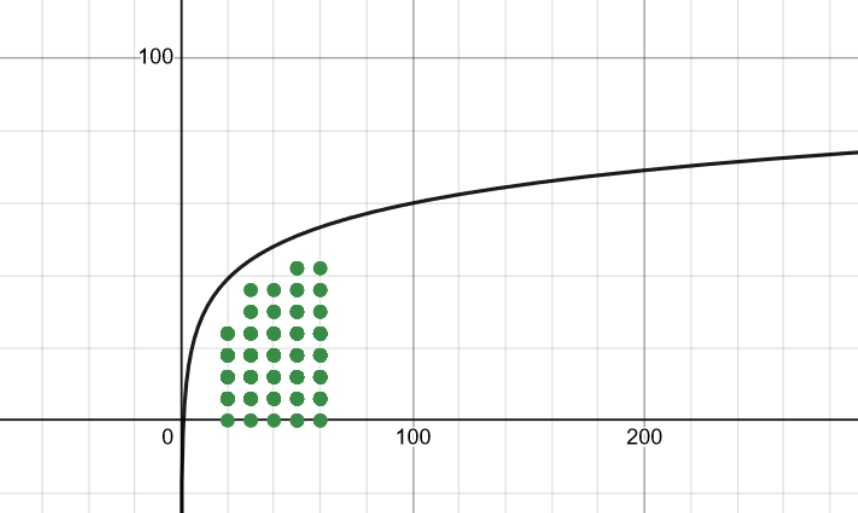
\includegraphics[scale=0.7]{euclides.jpg}
\caption{Gráfica del caso general}
\label{fig:universe}
\end{figure}

\begin{figure}[h!]
\centering
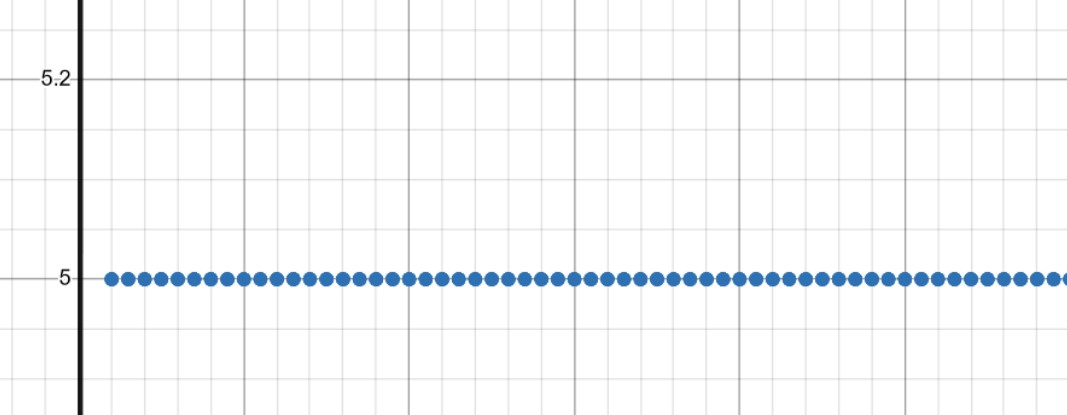
\includegraphics[scale=0.7]{mejor_caso_euclides.jpg}
\caption{Gráfica del mejor caso euclides}
\label{fig:universe}
\end{figure}

\begin{figure}[h!]
\centering
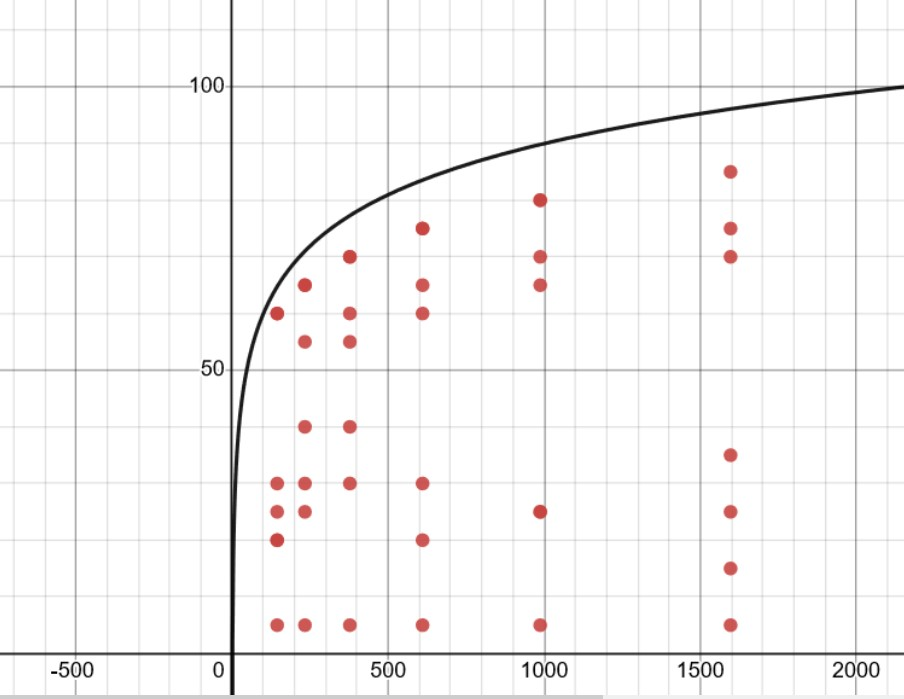
\includegraphics[scale=0.7]{peor_caso_euclides.jpg}
\caption{Gráfica del peor caso euclides}
\label{fig:universe}
\end{figure}

\clearpage

\section{Conclusiones}
Durante el desarrollo de esta practica la principal dificultad que se presento fue al momento de realiza la graficacion, mas precisamente al momento de definir las cotas superiores asintóticas y las cotas inferiores asintóticas, una vez resulto esto el resto fue mas sencillo, ahora bien, la interpretación que nosotros podemos darle a las gráficos en general es que para el primer Problema, en el análisis a posteriori la complejidad de nuestro algoritmo es lineal tanto para el mejor como el peor caso y esto no lo dicta la gráfica. Y para nuestro segundo algoritmo la complejidad es constante para el mejor caso y logarítmica para el peor caso, cabe resaltar que estas interpretaciones se hacen en base a lo que se observa en las respectivas gráficas. 
\\
\\
Conclusión Martinez Lopez Sebastian:\\
Observamos que existen varios algoritmos para dar solución a un solo problema en especifico, con esto observamos que dependiendo de los diferentes requerimientos que nos hagan o requiera el programa es el algoritmo que podemos usar, ya que como paso en esta practica el algoritmo puede tener tres complejidades diferentes para diferentes casos y con esto podemos hacer que nuestro programa sea mas eficiente dependiendo del tipo de caso en el cual vaya a estar trabajando. 
\begin{figure}[h!]
\centering
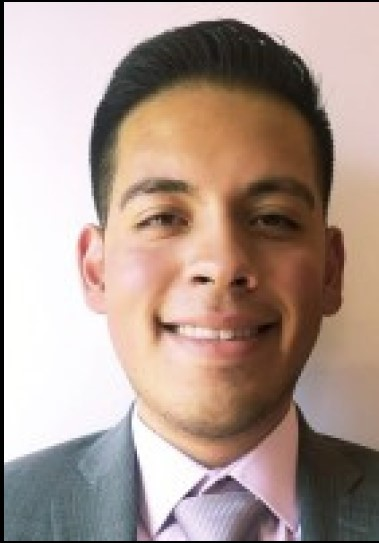
\includegraphics[scale=0.7]{seb1.jpg}
\caption{}
\label{fig:universe}
\end{figure}
\\
Conclusión Ramirez Resendiz Luis Roque:\\
Podemos darnos cuenta que un solo algoritmo puede cambiar su complejidad dependiendo el caso en el que se encuentre y de esta manera nosotros podemos valorar y hacer un análisis a fondo sobre dicho algoritmo, permitiéndonos compararlo con otros algoritmos que resuelvan el mismo problema e implementando el algoritmo que mas nos convenga, obviamente basándonos en las necesidades o el para que requiramos el algoritmo.
\begin{figure}[h!]
\centering

\includegraphics[scale=0.7]{luis1.jpg}
\caption{}
\label{fig:universe}
\end{figure}

\section{Bibliograf\'ia}
\\
Notación big O. (s/f). Pablocianes.com. Recuperado el 7 de septiembre de 2022, de https://pablocianes.com/notacion-big-o/

Notación Omega grande (Big-Ω). (s/f). Khan Academy. Recuperado el 7 de septiembre de 2022, de https://es.khanacademy.org/computing/computer-science/algorithms/asymptotic-notation/a/big-big-omega-notation

Notación θ grande (Big-θ). (s/f). Khan Academy. Recuperado el 7 de septiembre de 2022, de https://es.khanacademy.org/computing/computer-science/algorithms/asymptotic-notation/a/big-big-theta-notation

(S/f-a). Rae.es. Recuperado el 7 de septiembre de 2022, de https://dle.rae.es/algoritmo

(S/f-b). Rae.es. Recuperado el 7 de septiembre de 2022, de https://www.rae.es/dpd/a%20posteriori

(S/f-c). Rae.es. Recuperado el 7 de septiembre de 2022, de https://www.rae.es/dpd/anterior

\medskip



\end{document}
